\documentclass{article}
\usepackage{graphicx, amsmath}
\graphicspath{ {./images/} }


\title{Supply \& Demand Classwork Solutions}
\author{Principles of Microeconomics}
\date{\today}

\begin{document}

\maketitle

\begin{enumerate}

\item False -- After the increase in demand, the market will tend towards equilibrium (because we're assuming perfect competition) which means that quantity supplied will equal quantity demanded at the new, higher equilibrium quantity.

 	\begin{figure}[h]
	\centering
	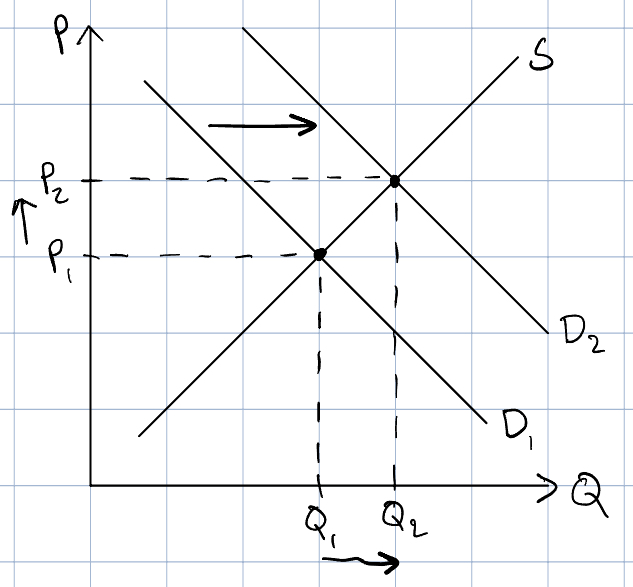
\includegraphics[width = 0.5\textwidth]{problem1}
	\end{figure}

\item

	\begin{enumerate}
	
	\item $P^* = 6$ and $Q^* = 81$
	
	\item If the actual price in the market were above the equilibrium price, there would be a surplus, so producers would cut their prices in order to attract more buyers.
	
	\item If the actual price were below the equilibrium price, there would be a shortage, so buyers would bid up the price in order to secure one of the pizzas. 
		
	\end{enumerate}

\newpage
	
\item People's taste for oranges will increase after the discovery about diabetes, so the demand curve will shift right, and the new fertilizer is a technological advancement that will shift the supply curve right. After the two shifts, the equilibrium quantity will unambiguously increase, but the change in equilibrium price is ambiguous.

	\begin{figure}[h]
	\centering
	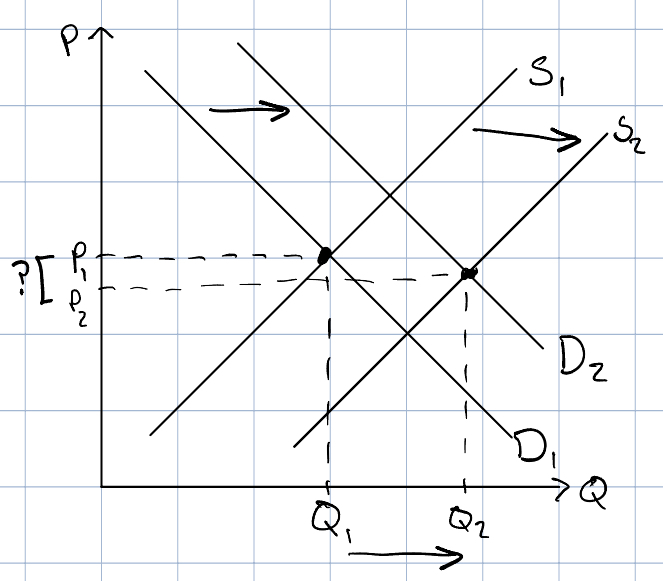
\includegraphics[width = 0.5\textwidth]{problem3}
	\end{figure}

\item

	\begin{enumerate}
	
	\item A fall in the price of flour could be responsible. Since flour is an input to bagels, a fall in the price causes the supply of bagels to shift right. That increases the equilibrium quantity and decreases the equilibrium price of bagels. Since bagels and cream cheese are complements, a decrease in the price of bagels causes the demand for cream cheese to shift right. That increases the price of cream cheese.
	
	\begin{figure}[h]
	\centering
	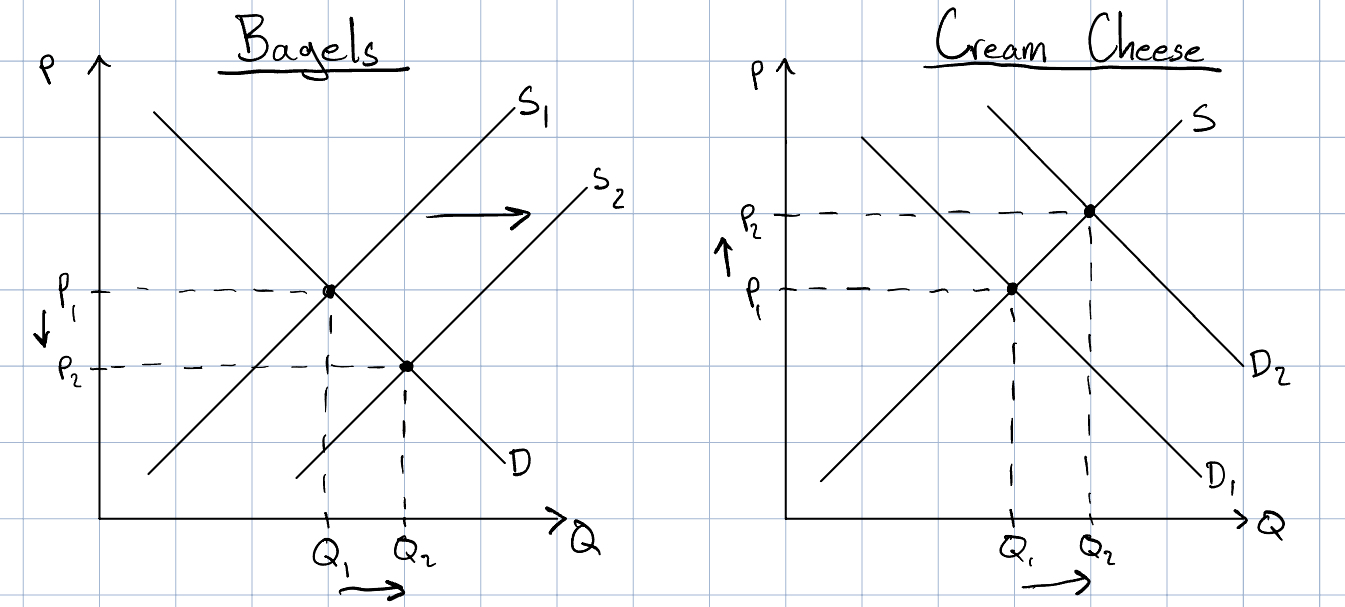
\includegraphics[width = \textwidth]{problem4a}
	\end{figure}
	
	\item A rise in the price of milk could be responsible. Since milk is an input to cream cheese, an increase in price causes the demand for cream cheese to shift left. That increases the equilibrium price of cream cheese. Since cream cheese and bagels are complements, an increase in the price of cream cheese causes the demand for bagels to shift left. That decreases the equilibrium quantity of bagels.
	
	\begin{figure}[h]
	\centering
	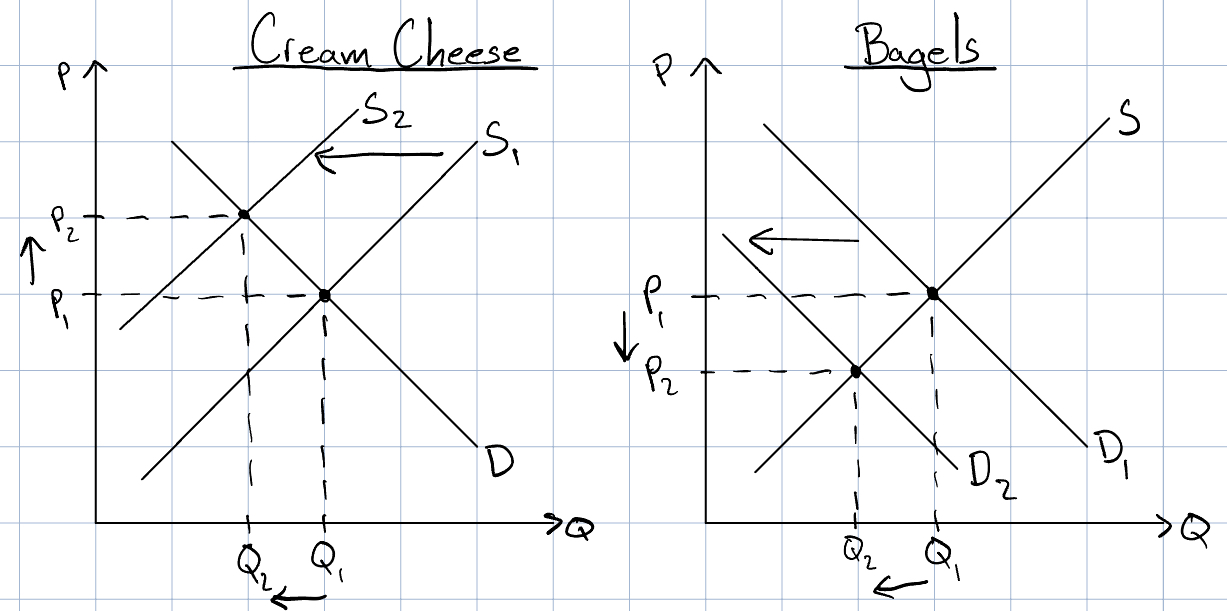
\includegraphics[width = \textwidth]{problem4b}
	\end{figure}
	
	\end{enumerate}
	
\item

	\begin{enumerate}
	
	\item The supply curve is vertical which might be because the number of seats in the baseball stadium is fixed.
	
	\item $P^* = 8$ and $Q^* = 8,000$.
	
	\item 
	
	\begin{center}
	\begin{tabular}{c c c}
	\textbf{Price} & \textbf{Quantity Demanded} & \textbf{Quantity Supplied} \\
	\hline
	\$4 & 10,000 + 4,000  = 14,000 tickets & 8,000 tickets \\
	8 & 8,000 + 3,000  = 11,000 & 8,000 \\
	12 & 6,000  + 2,000 = 8,000 & 8,000 \\
	16 & 4,000 + 1,000 = 5,000 & 8,000 \\
	20 & 2,000 + 0 = 2,000 & 8,000
	\end{tabular}
	\end{center}
	
	$P^* = 12$ and $Q^* = 8,000$
	
	\end{enumerate}
	
%\item Since hot dogs and ketchup are complements, an increase in the price of hot dogs causes demand for ketchup to shift left which in turn causes the equilibrium quantity to decrease. Tomatoes are an input to ketchup, so a smaller equilibrium quantity of ketchup means there are fewer buyers of tomatoes, and that causes demand for tomatoes to shift left and the price of tomatoes to fall. Tomatoes are also an input to tomato juice, so the lower price of tomatoes causes the supply of tomato juice to shift right and the price of tomato juice to fall (Note: you might be tempted to 

\item
	\begin{enumerate}
	
	\item
	\begin{gather*}
	Q_D = Q_S \\
	144 - 12P^* = 16 + 4P^* \\
	160 = 16P^* \\
	10 = P^* \\
	Q^* = 16 + 4P^* \\
	Q^* = 16 + 4(10) \\
	Q^* = 56
	\end{gather*}
	
	\item First, we need to calculate foreign demand before the increase:
%	\item The key to this problem is recognizing that $Q_D = Q_{D,Dom} + Q_{D,For}$ because market demand is equal to the sum of individual or component demands. Eventually, we'll need to set $Q_D = Q_S$ to find the equilibrium. $Q_S$ doesn't change, so we just need to calculate $Q_D$ after the increase in foreign demand. To do that, we first need to calculate foreign demand before the increase:
	\begin{align*}
	Q_D &= Q_{D,Dom} + Q_{D,For} \\
	144 - 12 P &= 80 - 8P + Q_{D,For} \\
	64 - 4P &= Q_{D,For}
	\end{align*}
	
	Next, we need to calculate market demand after the increase in foreign demand:
	\begin{align*}
	Q_D' &= Q_{D,Dom} + 1.5Q_{D,For} \\
	Q_D' &= 80 - 8P + 1.5(64 - 4P) \\
	Q_D' &= 80 - 8P + 96 - 6P \\
	Q_D' &= 176 - 14P
	\end{align*}
	\end{enumerate}
	
	Now, we can calculate the equilibrium price:
	\begin{align*}
	Q_D' &= Q_S \\
	176 - 14P' &= 16 + 4P' \\
	160 &= 18P' \\
	\frac{80}{9} &= P'
	\end{align*}

\end{enumerate}

\end{document}